%Autores: Prof. Me. Phyllipe Lima
%         Daylon Ramos da Silva
%Contato: phyllipe@inatel.br 
%         biblioteca.pesquisa@inatel.br
%Modelo para escrita de artigos científicos para o curso de Pós-Graduação em Desenvolvimento de Aplicações para Dispositivos Móveis e Cloud Computing do INATEL - Instituto Nacional de Telecomunicações. 
%Este template LaTeX é uma adaptação do modelo doc desenvolvido pelos professores Carlos Ynoguti e Dayan Guimarães

%Se você é novo no latex, um bom lugar para começar é
%https://pt.overleaf.com/learn
\documentclass[10pt,twocolumn]{article} 
%Use esse arquivo para incluir novos pacotes

\usepackage[%usado para determinar medidas
top=5mm,
bottom=1.78cm,
left=1.65cm,
right=1.65cm,
includeheadfoot
%showframe
]{geometry}

%\usepackage[justification=centering]{caption}
\usepackage{inatel}%carregar algumas estilizacoes do inatel
\usepackage{times}
\usepackage{enumitem}%redefinir espacos itemize
\usepackage{graphicx}
\usepackage{url,hyperref}
\usepackage[utf8]{inputenc}
\usepackage{float}%mais controle para manipular figuras
\usepackage{caption}%manipular legenda da figura e tabela
\usepackage{mathtools}%equacoes
\usepackage[hang,flushmargin]{footmisc} 
\usepackage{xcolor}
\usepackage{wrapfig} %usado para envolver figura com texto
%\usepackage[portuguese]{babel}
\usepackage{etoolbox}
\usepackage{adjustbox}%mais controle para ajustar tamanho da tabela
\usepackage{comment}%ambiente para comentario
\usepackage{relsize} %usado por comandos \mathlarger
\usepackage{fancyhdr}
\usepackage{everypage}

%Referencia bibliografica
\usepackage[
    style=numeric,
    sorting=none,
    maxbibnames=10]{biblatex}
\addbibresource{referencia.bib}

%Idioma. Use "english" para trabalhos em inglês
\usepackage[brazil]{babel}
%Ajustes na legenda da figura. Incluindo espacamento apos a legenda
\captionsetup[figure]{labelformat={default},labelsep=period,font=footnotesize, name=\footnotesize{Fig.},justification=raggedright,singlelinecheck=false,belowskip=-0.9\normalbaselineskip}
%\pagenumbering{gobble}

%Ajustes na legenda da tabela. 
%Ajustes na legenda da tabela. 
\captionsetup[table]{labelformat={default},labelsep=newline,font={sc,footnotesize},justification=centering,singlelinecheck=false}


%%%%%%%%%%%%%%%%%%%%%%%%%%%%%%%%%%%%%%%%%%%%%%%%%%%%%%%%%%%%%%%%%%%%%%%%%
%    Configuracaoes de Idioma
%    Considerando babel = brazil
%%%%%%%%%%%%%%%%%%%%%%%%%%%%%%%%%%%%%%%%%%%%%%%%%%%%%%%%%%%%%%%%%%%%%%%%% 

\addto\captionsbrazil{
  \renewcommand{\abstractname}{Abstract}
  \renewcommand{\tablename}{TABLA}
  \renewcommand{\ref}{{Referencias}}
}

%considerando babel = english
\addto\captionsenglish{
  \renewcommand{\tablename}{TABLE}
   \renewcommand{\ref}{{Referencias}}
}


%Configurações do Cabeçalho!
\fancypagestyle{first}{%
    \fancyhf{} % limpa os campos
    \chead{ \textcolor{black!50}{\textbf{
    \textcolor{red}{OpenCV} Spatial AI Competition sponsored by Intel \\
    \textcolor{red}{JULIO} DE 20\textcolor{red}{20} 
    \vspace*{2\baselineskip}
    }}}
    \rhead{\textcolor{black!50}{\textbf{
    %e-ISSN 2595-8186
    }}}
}

\AddEverypageHook{
    \ifnum\value{page}=1%
        \setlength{\headheight}{50pt} 
    \else
        \setlength{\headheight}{0pt} 
    \fi}
    
\renewcommand{\headrulewidth}{0pt}
\renewcommand{\footrulewidth}{0pt}


%contador de autores
%o comando dever ser \contAutor
\newcounter{contador}
\newcommand\contAutor{\stepcounter{contador}\thecontador}


\AtBeginBibliography{\small}
\AtBeginDocument{\pagestyle{empty}}

%Inicio do documento
\begin{document}

\title{\Huge \bf Monitoreo Automático de índice condición corporal en bovinos usando cámara de profundidad espacial con inteligencia artificial con el fin de incrementar el nivel de tecnificación en los pequeños productores.}

\author{\large 
Darío Mendoza\textsuperscript{\contAutor}, Fernando Recalde\textsuperscript{\contAutor}, Marcelo Ortiz\textsuperscript{\contAutor}, Christopher Obando\textsuperscript{\contAutor}}

\maketitle
\thispagestyle{first}
%\noindent\blfootnote{Trabalho de Conclusão de Curso apresentado ao  %Prof. (XXXXX). Trabalho aprovado em XX/20XX.}

\setlength{\tabcolsep}{5pt}

\section{Introducción}

Aqui va la introducción.

\vspace{5mm} %5mm vertical space
\section{Antecedentes}

El ganado contribuye a casi el 40\% de la producción agrícola total en los países desarrollados y el 20\% en los países en desarrollo, en Ecuador el sector del ganado vacuno constituye un total de 4.31 millones de cabezas a nivel nacional del total existente al 2019.
En Ecuador la producción de leche ronda los 6,65 millones de litros anuales con un rendimiento de 10,84 litros/vaca lo cual representa más de 1600 millones en ventas anuales para el país \cite{Encuesta}.

El 92\% de la ganadería ecuatoriana proviene de la agricultura familiar por lo que la forma de gestionar la alimentación de sus bovinos es de forma artesanal y no son asesorados por personal técnico calificado, las vacas son alimentadas  con vegetación natural con niveles nutricionales muy bajos y residuos de cultivos, con bajo o nulo monitoreo de sus niveles de nutrición, lo que ocasiona que se presenten pérdidas en la producción.   

\vspace{5mm} %5mm vertical space
\section{Índice condición corporal en bovinos}
Uno de los principales factores que debe tomar en cuenta el productor ganadero, es controlar la nutrición en sus animales, el método más conocido para identificar el nivel de nutrición en bovinos es la monitoreo de la condición corporal, consiste en evaluar mediante una apreciación visual  las reservas corporales de grasa y músculo, bajo un patrón preestablecido al que se le ha dado valores numéricos arbitrarios, estos valores están ordenados conforme a una escala que en las razas británicas y  continentales va de 1 a 5 y en las índicas y sus cruzas de 1 a 9 \cite{ImportanciaCria}. 

Las investigaciones indican que existe un fuerte vínculo entre la condición corporal de una vaca y su rendimiento reproductivo, está relacionada con muchos aspectos críticos de la producción por ejemplo ayuda a los productores a tomar decisiones de gestión con respecto a la calidad y cantidad de alimento necesarios para garantizar la salud, optimizar la producción y reproducción \cite{Eversole2014BodyCows,Arias2008FactoresLeche}.

\vspace{5mm} %5mm vertical space
\subsection{Relación entre condición corporal y eficiencia reproductiva}

El porcentaje de eficiencia reproductiva está directamente relacionado con dos factores: el número de parto y la condición corporal.  (Tabla 1). Se considera que vacas con una condición corporal mayor a 3, tienen un 29\% mayores tasas de preñez  comparada con vacas con una condición corporal menor a 2.5 \cite{RelacionHolstein}. La pobre condición corporal afecta no solo la tasa de preñez sino el intervalo entre partos (IEP) y la edad del ternero al destete \cite{RelacionHolstein}.

\begin{table}[h]
\caption{Relación del parto y la condición corporal con
tasas de preñez (\%)}
\label{tab:tabla1}
\begin{adjustbox}{max width=\textwidth}
\begin{tabular}{| c | c | c | c | }
\hline
\multicolumn{1}{ |c| }{Parto} & \multicolumn{3}{ |c| }{Condición corporal} \\ \hline
N  & $<2.0$ & $2.5$ & $>3.0$ \\ \hline
1 & 20 & 53 & 90 \\
2 & 28 & 50 & 84 \\
3 & 23 & 60 & 90 \\
4-7 & 48 & 72 & 92 \\
$> 8$ & 37 & 67 & 89 \\ \hline
\end{tabular}
\end{adjustbox}
\end{table}

Sin embargo, el método actual para medir BCS en granjas lecheras modernas todavía es manual. El BCS manual lleva mucho tiempo en granjas grandes y requiere mano de obra capacitada \cite{Halachmi2013AutomaticImaging}. Otro problema asociado con el puntaje manual es la subjetividad del proceso, el puntaje depende de la persona que realiza la medición.a pesar de lo anteriormente mencionado  menos del 5\% de las granjas lecheras de los EEUU han adoptado esta práctica en la cadena de producción \cite{Azzaro2011ObjectiveImages}.

Las principales razones que desalientan el uso de las técnicas de evaluación de BCS son la falta de informes computarizados, la  subjetividad y el tiempo de capacitación de técnicos en la granja. Et Al \cite{Schroder2006InvitedThickness} sugieren que un BCS automático requiere menos tiempo, es menos estresante para el animal, más objetivo y consistente, y posiblemente sea más rentable. Por lo tanto, el desarrollo de un dispositivo automático basado en imágenes digitales para monitorear BCS es de interés económico.

\vspace{5mm} %5mm vertical space
\subsection{Relación entre condición corporal y eficiencia reproductiva}

El porcentaje de eficiencia reproductiva está directamente relacionado con dos factores: el número de parto y la condición corporal.  (Tabla 1). Se considera que vacas con una condición corporal mayor a 3, tienen un 29\% mayores tasas de preñez  comparada con vacas con una condición corporal menor a 2.5 \cite{RelacionHolstein}. La pobre condición corporal afecta no solo la tasa de preñez sino el intervalo entre partos (IEP) y la edad del ternero al destete \cite{RelacionHolstein}.

\vspace{5mm} %5mm vertical space

\printbibliography

\section*{Autores}
%Lembrar de reiniciar os contadores de autores aqui com o comando abaixo \setcounter{contador}{0}
\setcounter{contador}{0}

\begin{wrapfigure}{l}{0.17\textwidth}
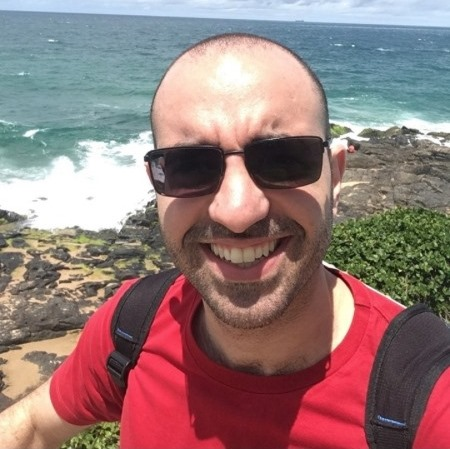
\includegraphics[trim= 0 2 0 0,clip,width=0.16\textwidth]{figuras/autor1.jpg}
\end{wrapfigure}

    \textbf{Dario Mendoza\textsuperscript{\contAutor}} Ingeniero en Mecatrónica graduado en - Universidad de las Fuerzas Armadas ESPE. Doutorando em Computação Aplicada pelo INPE - Instituto Nacional de Pesquisas Espaciais, na área de Engenharia de Software realizando estudos sobre metadados através da análise estática de código fonte e MSR (Mining Software Repositories). Mestre em Ciência da Computação(2016) pela UNIFEI - Universidade Federal de Itajubá. Engenheiro de Telecomunicações(2011) pelo INATEL - Instituto Nacional de Telecomunicações.  Técnico em Telecomunicações(2006) pela Escola Técnica de Eletrônica - ETE "FMC". É professor auxiliar do INATEL, atuando nos cursos de Engenharia da Computação e Engenharia de Software. Tem interesse nas áreas de Engenharia de Software Empírica e Desenvolvimento de Jogos\newline
    
\begin{wrapfigure}{l}{0.15\textwidth}
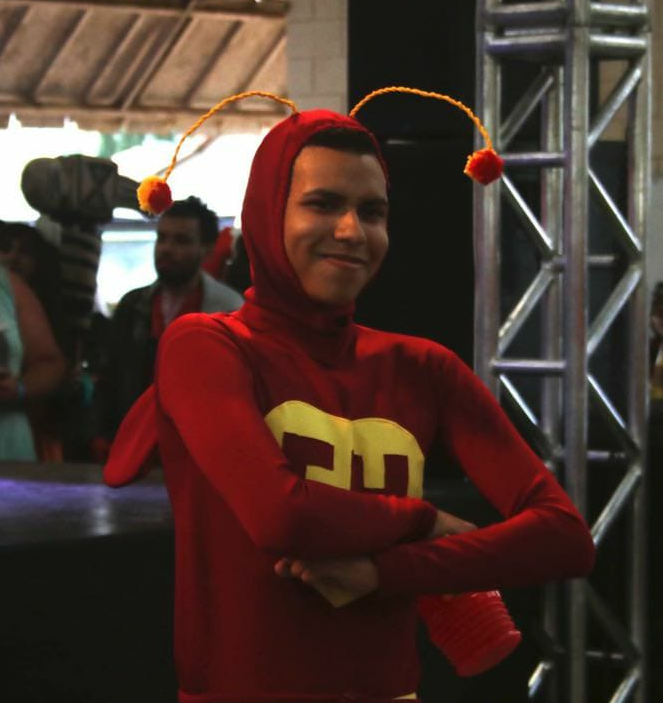
\includegraphics[trim= 0 2 0 0,clip,width=0.14\textwidth]{figuras/autor2.png}  
\end{wrapfigure}

   \textbf{Fernando Recalde\textsuperscript{\contAutor}} Ingeniero  graduado en - Universidad de las Fuerzas Armadas ESPE.é graduando em Tecnologia em Gestão de Telecomunicações pelo INATEL - Instituto Nacional de Telecomunicações. Tem interesse nas áreas de tecnologia, gestão e engenharia de produção.\newline

\begin{wrapfigure}{l}{0.15\textwidth}
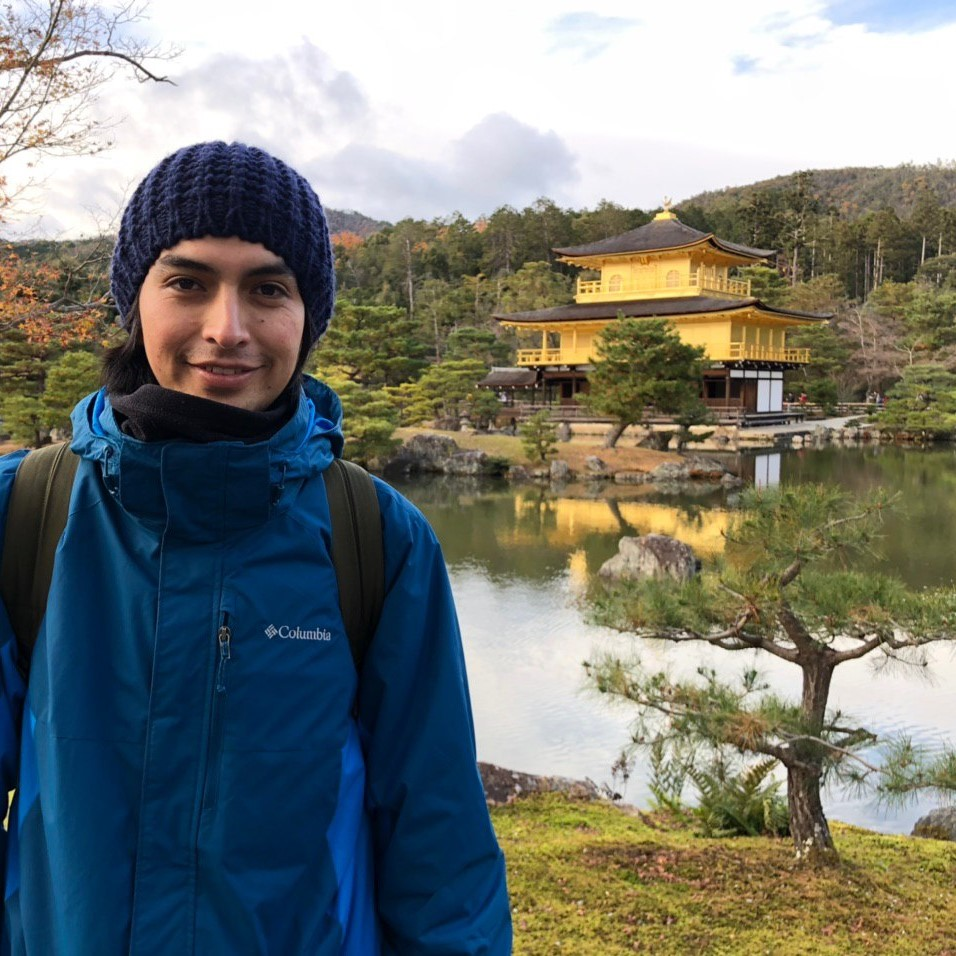
\includegraphics[trim= 0 2 0 0,clip,width=0.14\textwidth]{figuras/autor3.jpg}  
\end{wrapfigure}

   \textbf{Marcelo Ortiz\textsuperscript{\contAutor}} Ingeniero  en Mecatrónica graduado en - Universidad de las Fuerzas Armadas ESPE.\newline
   
\begin{wrapfigure}{l}{0.15\textwidth}
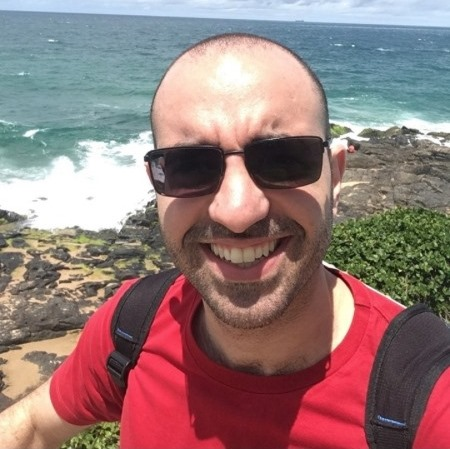
\includegraphics[trim= 0 2 0 0,clip,width=0.14\textwidth]{figuras/autor1.jpg}  
\end{wrapfigure}

   \textbf{Christopher Obando\textsuperscript{\contAutor}} Ingeniero  graduado en - Universidad de las Fuerzas Armadas ESPE.é graduando em Tecnologia em Gestão de Telecomunicações pelo INATEL - Instituto Nacional de Telecomunicações. Tem interesse nas áreas de tecnologia, gestão e engenharia de produção.
\end{document}